\documentclass[12pt]{beamer}
\usepackage{amsmath,amssymb,caption,float}
\usepackage[ruled,vlined]{algorithm2e}
\usetheme{AnnArbor}
\setbeamercolor{normal text}{bg=black!10}

\SetKwInOut{Input}{Input}
\SetKwInOut{Output}{Output}
\SetKwProg{Fn}{Function}{\string:}{end}
\SetKwFunction{parse}{parse}

\begin{document}
\title{How to Parse Input}
\subtitle{VE482 Project1 Presentation}
\author{Group 5, Yihua Liu, Boqun Li, Yu Xiao}
\institute{UM-SJTU Joint Institute}
\date{\today}
\begin{frame}
    \titlepage
\end{frame}


\section{Useful C Library}
\begin{frame}{$<$string.h$>$}
    \begin{itemize}
        \item This is the C library includes most of the functions that operate on C strings.
        \item For C strings comparison, we have:
            \begin{itemize}
                \item \textbf{strstr()}
                \item \textbf{strcmp()}
            \end{itemize}
        \item For C strings partition, we have:
            \begin{itemize}
                \item \textbf{strtok()}
            \end{itemize}
    \end{itemize}
\end{frame}

\section{C Strings Comparison}
\begin{frame}{strstr()}
    \begin{block}{Declaration}
        char *strstr( const char *str, const char *substr )
    \end{block}
    A function that can tell whether a string contains a substring.\\
    \textbf{Parameters}
    \begin{itemize}
        \item $str$: pointer to the null-terminated byte string to examine
        \item $substr$: pointer to the null-terminated byte string to search for
Return value
    \end{itemize}
    \textbf{Return value} \\
    \ \ \ \ Pointer to the first character of the found substring in str, or a null pointer if such substring is not found. If substr points to an empty string, str is returned.
\end{frame}

\begin{frame}{strcmp()}
    \begin{block}{Declaration}
        int strcmp( const char *lhs, const char *rhs )
    \end{block}
    A function that can tell whether two strings are identical. \\
    \textbf{Parameters}
    \begin{itemize}
        \item $lhs$, $rhs$: pointers to the null-terminated byte strings to compare
    \end{itemize}
    \textbf{Return value}
    \begin{itemize}
        \item Negative value if lhs appears before rhs in lexicographical order.
        \item Zero if lhs and rhs compare equal.
        \item Positive value if lhs appears after rhs in lexicographical order.
    \end{itemize}
\end{frame}

\section{C Strings Partition}
\begin{frame}{strtok()}
    \begin{block}{Declaration}
        char *strtok( char *str, const char *delim )
    \end{block}
    A function that can spilt strings by certain delimiter. \\
    \textbf{Parameters}
    \begin{itemize}
        \item $str$: pointer to the null-terminated byte string to tokenize
        \item $delim$: pointer to the null-terminated byte string identifying delimiters
    \end{itemize}
    \textbf{Return value} \\
    \ \ \ \ Returns pointer to the beginning of the next token or a null pointer if there are no more tokens.
\end{frame}

\begin{frame}{strtok()}
    \textbf{Note} \\
    \ \ \ \ This function is destructive. It will replace every string matching $delim$ by '$\backslash0$'.\\
    \textbf{Example}
    \begin{figure}
        \centering
        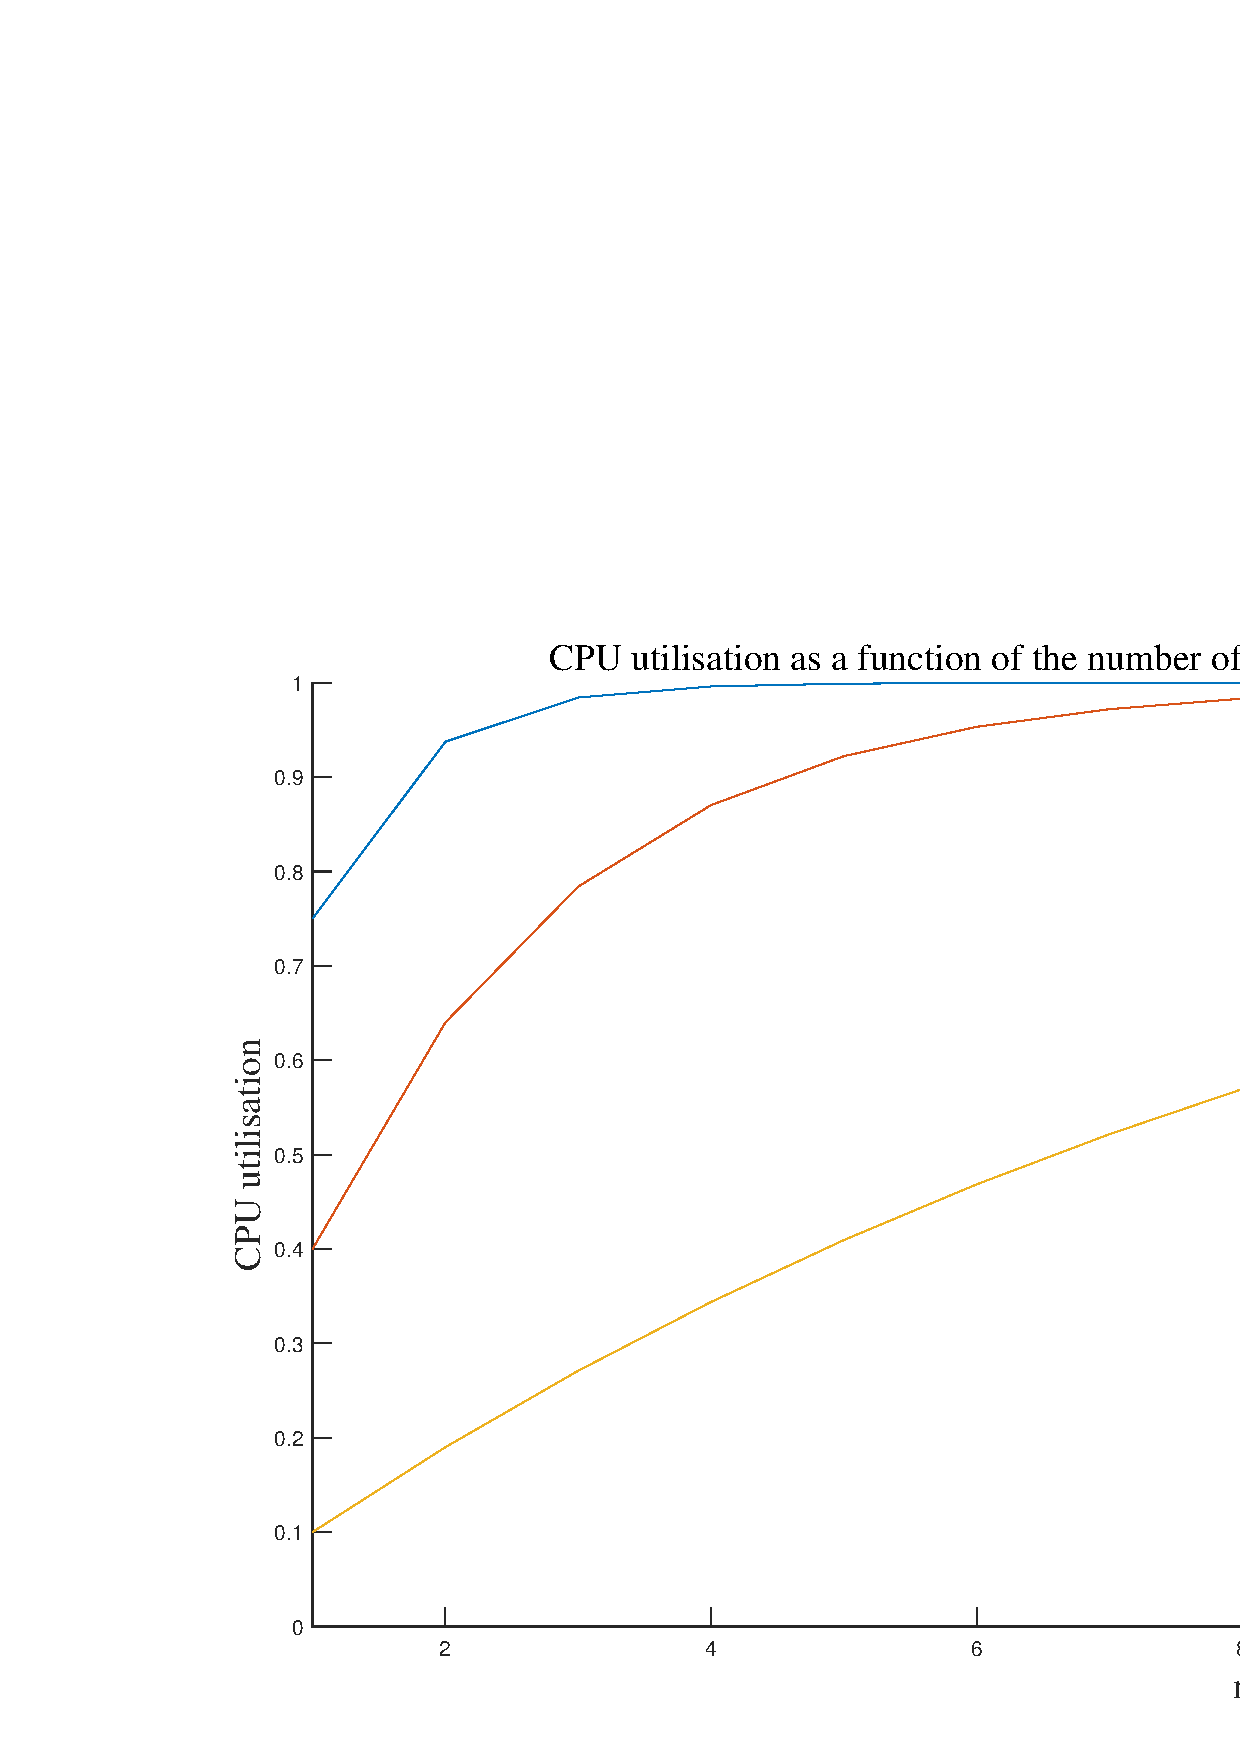
\includegraphics[width=11cm]{1.png}
        \label{fig:example_strtok}
    \end{figure}
\end{frame}

\begin{frame}{strtok()}
    \textbf{Result}
    \begin{figure}
        \centering
        \includegraphics[width=11cm]{2.png}
        \label{fig:result_strtok}
    \end{figure}
\end{frame}

\section{Parsing Method}
\begin{frame}{parse char by char}
\begin{enumerate}
    \item Use a pointer pointing to the address of command as iterator.
    \item Deal with one character in each iteration.
    \item Deal with pipe '$|$' seperately.
    \item there are several cases:
    \begin{enumerate}
        \item *iter = '\ '
        \item *iter = '$ > $'
        \item *iter = '$ < $'
        \item *iter = '$ > $' \&\& *(iter+1) = '$ > $'
        \item *iter is other normal character
    \end{enumerate}
\end{enumerate}
\end{frame}

\begin{frame}{parse\_v1()}
\scalebox{0.75}{
    \begin{algorithm}[H]
        \DontPrintSemicolon
        % \SetKwInOut{Input}{Input}
        % \SetKwInOut{Output}{Output}
        \Input{original command line \texttt{cmd}, empty list argv[][]}
        \Output{resulted char** argv list}
        \parse{char *cmd, char** argv}{\;
            $j\leftarrow0$,$i\leftarrow0$\;
            $char* iter \leftarrow cmd$\;
            \While{*iter}{
                \If{*iter == '\ '}{
                    $i\leftarrow i+1$, $j\leftarrow 0$;
                }
                \ElseIf{*iter == '$>$' }{
                    skip spaces\;
                    \While{next arg or end of line}{
                        $iter\leftarrow iter+1$\;
                    }
                }
                \ElseIf{ \dots}{\dots\;}
                \Else{
                    argv[i][j] = *iter\;
                    $j\leftarrow j+1$\;
                }
                $iter\leftarrow iter+1$\;
            }
        \Return{argv}
        }
        \caption{parse()}
    \end{algorithm}
}
\end{frame}

\begin{frame}{parse()}
    \begin{enumerate}
        \item redirection\_parse()
        \item Check whether \texttt{token[0] == '>'}
        \begin{itemize}
            \item Check whether \texttt{strlen(token) == 2 \&\& token[1] == '>'}
        \end{itemize}
        \item Check whether \texttt{token[0] == '<'}
        \item Check whether \texttt{token[0] == '|'}
        \item \texttt{token = strtok(NULL, token delimiters)}
    \end{enumerate}
    This method would pass all words to \texttt{execvp()} function until \texttt{'>', '<', or '|'}, so it is the same for cases with arguments and without arguments.
\end{frame}
\begin{frame}{redirection\_parse()}
\scalebox{0.75}{
    \begin{algorithm}[H]
        \DontPrintSemicolon
        \KwData{original command line \texttt{cmdln}}
        \KwResult{command line with all proper spaces added \texttt{parsedln}, token}
        \Begin{
            $j\leftarrow0$\;
            \For{$i\leftarrow1$ \KwTo \texttt{strlen(cmdln)}}{
                \tcc{Forward parsing}
                \If{\texttt{cmdln}[$i$]=$<$ {\bf or} $>$ {\bf or} $|$ {\bf and} \texttt{cmdln}[$i-1$]$\neq$' ' {\bf and not} two adjacent $>$}{
                    \texttt{parsedln}[$j$]$\leftarrow$' '\;
                    $j\leftarrow j+1$\;
                }
                \tcc{Backward parsing}
                \If{\texttt{cmdln}[$i-1$]=$<$ {\bf or} $>$ {\bf or} $|$ {\bf and} \texttt{cmdln}[$i$]$\neq$' ' {\bf and not} two adjacent $>$}{
                    \texttt{parsedln}[$j$]$\leftarrow$' '\;
                    $j\leftarrow j+1$\;
                }
            }
            token$\leftarrow$first word of \texttt{parsedln} separated by token delimeters\;
        }
        \caption{redirection\_parse}
    \end{algorithm}
}
\end{frame}



\section{}
\begin{frame}
    \begin{center}
        \Huge Thanks!
    \end{center}
\end{frame}
\end{document}
